
\chapter{Requirements and Architecture}
In order to come up with detailed requirements and a corresponding architecture an explorative process had to be used. The initial, overall objective was to createa general-purpose DDoS visualization system that focuses on data available in the DDoSDB dataset. In literature there one can find processes on how to derive an appropriate visualization for a defined problem, such as the following data analysis step from Marty\cite{appliedsecurityvisualization}:
\begin{enumerate}
    \item Define the problem to become aware of which questions need to be answered by the final visualization.
    \item Assess the available data to determine how it can be used and how it might need to be extended.
    \item Parse and filter the available data to extract the relevant information
    \item Determine which visual properties such as shape or size are needed
    \item Determine the view of the graph that was created in the previous step. This includes transformatinos such as scale or zooming.
    \item Interpret the graph and answer the initial question
\end{enumerate}

Since this process is targeted at solving a specific problem and our objective was the development of a general-purpose visualization system we adapted it as is described in the remaining sections of this chapter. First, we analysed the information that can be extract from various network captures from DDoSDB. This also included the determination of their scale and possible tools for data extraction. The outcome of this step was a general understanding on how the data needs to be parsed, aggregated and or filtered to create a general-purpose visualization system. This constitutes a "bottom-up approach" where we first analyse the data and parse it in the most generic way that enables the information to be used with as many visualizations as possible while still maintaining technical feasibility for large datasets.

>> How did we come up with requirements?? 

Given the requirements to such a system and the understanding of available information and scale of the data sets we then created the initial architecture.

\section{Analysis of Data Sets}
Before defining detailed use-cases available data was explored to determine feasible requirements, visualizations and implementations. To be more specific, a proof of concept data mining tool was built to answer the questions that needed to be cleared before progressing. The following subsections describe the questions that were supposed to be answered by the Proof of Concept and their results. With these results in hand an initial brainstorming session about possible use-cases done we were able to synthesize all information. The result is the use-cases that are supposed to be as abstract as possible to be inline with the overall objective of building a general-purpose platform whose prototypical implementation can be considered technically feasible.
The scope of the POC was to write a data miner that can provide at least the same functionality as can be obtained from the fingerprints that are available in DDoSDB.


\subsection{Libraries and Tooling}\label{librariesandtooling}

\textit{What libraries exist and which features do they provide?}   

   Different tools and libraries were evaluated such as tsflow a CLI tool, node\_pcap a JavaScript based wrapper around libpcap and pkts, which is a parser written purely in Java.
    The Java library seemed to provide the best performance but for simple prototyping the Node.js based library was chosen. It provided parsing of protocols up until the application layer (app layer not included?) and heavily relies on libpcap. Support for stream processing in Node.js and the event-driven nature of JavaScript made the implementation feel quite "natural" and easy to read.
    Using node\_pcap it was possible to create the same information as provided in the DDoSDB dataset. Initially we suspected that we would run into performance problems especially when using very large datasets, which turned out not to be the case. This was due to the ease of implementation using stream processing which would make the POC scale easier with large sets. The duration of mining was also surprisingly good. This was tested by profiling the application when mining the largest dataset we could find on DDoSDB. This revealed that it only took seconds and that a majority of time was spent in the native libpcap module. This can be explained in that node\-pcap is merely a wrapper around libpcap. Figure \ref{fig:profiling} shows the result of profiling the miner. We thus conclude that node\_pcap provides all required functionality and that writing the miner in a way that it scales to larger datasets will be straightforward.
    
    \begin{figure}[profiling]
    \centering
    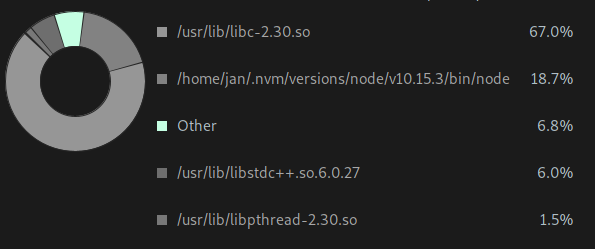
\includegraphics[width=10cm]{images/profiling.png}
    \caption{Profiling the data miner with a 15MB network capture as input.}
    \label{fig:profiling}
\end{figure}

> Describe implementation for further reeferences
    
\subsection{Information granularity?}
\textit{What information is contained in the network capture data sets? Which protocols and levels are sensible to analyse?
}

As a source for possible datasets the DDoSDB database was chosen. The reason for this are the features it provides as stated in section \ref{ddosdb}. The main benefit was direct access to network capture files that are already classified and in various sizes. This made it easy to see which information can be obtained in different attacks, such as for example, the payload of an ICMP packet. Since it is very simple to create a network capture of a "normal state" it was simple to compare the analysis of both cases.
Using the network capture files and a WHOIS service with the implemented proof of concept we were able to recreate the fingerprints from DDoSDB along with some additional information. The remainder of this section describes the data that can be extracted and an assessment if and how it is useful to collect for a visualization system:
\subsubsection{PCAP}
The first packet is a PCAP wrapper around the network-access level packet. It contains information such as \textbf{packet length} and a \textbf{timestamp} in seconds and microseconds. It is worth to note that this data needs to be interpreted on the place where it was captured.
Both of these properties are important to gather in order to compute the average packet length and attack start and duration.
\subsubsection{Network access layer}
In the payload of the PCAP packet one usually finds an Ethernet packet. Other network-layer protocols would be possible but only Ethernet packets were observed in the network captures.
The following information can be extracted from Ethernet packets:
\begin{itemize}
\item Destination and Source MAC addresses
\item Network-layer protocol
\item vlan ID
\end{itemize}
Since the information is very low-level and does not convey important semantics about any of the most frequent DDoS attack types we don't consider any of the information useful to store except for the Internet protocol that would be considered in the next subsection.
\subsubsection{Internet layer}
This was the first layer where multiple protocols were observed, naturally those would be IPv4 and IPv6. The network captures within DDoSDB were almost entirely based on IPv4 which is why this was focused on:
\begin{itemize}
\item Source and destination address
\item Version
\item TTL
\item DiffServ
\item Length
\item Transport-layer protocol
\item Version
\item checksum
\end{itemize}
     Except for checksums and transport-layer protocol, which was considered on the next layer, all properties could be sensible to mine.
     For some attacks the number of involved source addresses was very large, so large that fingerprints from DDoSDB would easily be larger than five megabytes. The problem with that is that it is difficult to work with in a front-end web application and it would be hard to visualize. For datasets that exceed some threshold of number of IP addresses aggregation would likely be required. This aggregation could be done based on arbitrary prefix aggregation, country or autonomous system.
     Other properties that are also sensible to aggregate would be TTL and length.
     \subsubsection{Transport layer}
In the transport layer two protocols were frequently observed: UDP and TCP.
Common to the two are the following fields:
\begin{itemize}
    \item Source and destination port
    \item Checksum
\end{itemize}
The packets using the TCP protocol also showed the following fields:
\begin{itemize}
    \item Acknowledgement number
    \item Sequence number
    \item Header length
    \item All six single-bit flags
    \item Window size
    \item Urgent Pointer
\end{itemize}
Source and destination port are definitely valueable to gather information on the application protocol being attacked. The flags would also be easy to aggregate over and give insight over the TCP state.

\subsection{Application layer}
The library that was used to parse packets does not contain a parser for application-level protocols. This means that to analyse this layer one has the protocol number and a buffer containing the payload. Perhaps it is already enough to aggregate over the type of protocols used. However the final implementation should definitely be easily extendable with new parsers for such protocols. For example, Node.js offers a performant and widely used HTTP parser which could be used to further gain insight about the application-level attack.
     
    \subsection{Scale and Schema of data}\label{scaleandschema}
\textit{    Are there consequences of the size and schema of the data with respect to visualizations? Can some technical challenges be determined?
}

    The reason why this question needs to be answered before designing visualizations is that depending on the size and distribution of the attributes that need to be visualized the visualization will either provide little value or be technically difficult. For example, consider an attack with 100'000 source IP addresses. Storing and fetching these addresses from a server to a web application will be taxing. Even if this were possible, there will hardly be a visualization that will provide insight while visualizing all 100'000 IP addresses. The answer to this question should define if aggregation of such attributes needs to be done and how.
    This is a technical challenge that can be taken for granted since network capture are technically unbound in size. This will also imply technical challenges for the mining of the source data since not the whole source and analysed data can be kept in memory.
    These challenges were observed while implementing the proof of concept. We assume that the following countermeasures will become important:
    \begin{itemize}
    \item     Applying \textbf{Big data techniques} to mine the source data will be very important to guarantuee that the data miner is technically capable of handling very large network capture files
\item Just looking at the fingerprints of the larger network captures in DDoSDB reveals that some of these JSON files are multiple megabytes in size. This both technically challenging to transfer and render and hard to interpret. However not only the size of these summaries is a problem, the fact that all information is contained in a single JSON file would lead to overfetching when used for different visualization. Overfetching refers to the problem of having to retrieve more data than being required by the client. Our solution to reducing the size and getting rid of overfetching is to create different resulting files for different visualizations. In a sense we would try to "\textbf{fan out}" the results over multiple files for improved scalability. For example, this could mean that for a time-series analysis of an attack we would create fixed-sized intervals and then create JSON files for each time interval. For other visualizations that would deal with more abstracted information we would also create single JSON files that have the only purpose to be used in that visualization. For example, a visualization a bar chart showing the top five autonomous systems used in an attack would only have to fetch a very small, dedicated JSON file containing said information.
\item Another solution to the aforementioned dilemma with very large results is to \textbf{aggregate} them. Ideally, this should be possible in a dynamic and user-defined way. For example, if an attack is executed from five source IP addresses, then this is technically possible and sensible to store as result and show in a visualization. However for hundreds or thousands of IP addresses either this visualization should be disabled or the underlying data could be aggregated to larger prefixes.
\item To enable the threshold where data will be aggregated more aggressively such a \textbf{user input} has to be implemented into the frontend of the webapplication.
\item Using a WHOIS service to query additional data about the source IP addresses does not scale up if more than a few thousand IP addresses need to be analysed. This is due to many WHOIS service providers being unwilling to deal with bulk requests of this size. Additionally, such requests would increase the duration of the data mining since it has to be transferred over the network. A local database needs to be considered as described in \ref{enrichingthedata}
\end{itemize}
    
    \subsection{Enriching the data}
\label{enrichingthedata}    \textit{Given the information that can be extracted, how can it be enriched? Which information makes sense to complement the network capture information with and how can it be obtained?}
    
In order to rebuild the functionality provided by the DDoSDB data miner, we need to provide the country and autonomous system number (asn) for each source IP address.
In the proof of concept implementation we used a WHOIS service provided by Team Cymru. This service supports bulk requests for WHOIS requests but is only willing to answer requests containing "(..) a few thousand" IP addresses \cite{teamcymru}. This along with the latency introduced by fetching the results over the network make this solution impracticable. For this, we intend to use the Geolite2 databases which are often used for geolocation of IP addresses. These datasets are interesting to us since they can be used locally and they have different datasets through which we could retrieve the ASN, country, city and belonging prefix for a source IP address \cite{geolite2}.

    
    \subsection{Aggregating the data} 
\textit{Given the information that can be extract how can or does it need to be aggregated?
}    

Section \ref{scaleandschema} described the necessity to aggregate in order to improve technical scalability and to make the visualizations sensible.
To visualize information with little abstraction, such as for example the source IPs for a certain time period, we will create a small data set containing just the relevant properties for that time interval.
For information with higher abstraction, such as for example visualizing overall metrics we follow the same strategy of creating a dataset for the visualization.
    \subsection{Fitting visualizations}
\textit{Given all the information that can be obtained, which visualizations are sensible?
}

We already established that the datasets need to be decoupled depending on visualization. To build a general purpose visualization platform it would be a good strategy to build a data miner that can easily be extended and then build visualizations and parsers for the most common attack types.
    \subsection{Constraints} 
\textit{Which constraints on the user input make sense? Which data sets make sense (e.g. location of recording)
}

If the application can deal with large datasets there should still be a limit for the size of input files since we don't know in which setting the application would be used. We think it makes sense to allow a user to define such a threshold in the application. Other constraints that are related to the visualizations, for example hiding certain outliers should be considered when designing the visualization.
In a first step it makes sense to write parsers only for network capture files, ideally from the DDoSDB database.
    
    \subsection{Frequent problems described in literature} 
    \textit{Literature describes that frequent problems are "Incomplete Information" and "Source / Destination Confusion". Are such problems relevant and if yes how can they be mitigated?}
    
    Detecting whether a dataset is incomplete is quite a difficult task since the proposed solution is not supposed to act as a classification or intrusion detection system. We therefore have to assume that we work with sane network capture files, which seems fair? since this data was already pre-processed by the DDoSDB\-cli and since network capture files are considered as rawest, compared to for example flow capture files \cite{appliedsecurityvisualization}.
    What is likely to happen and feasible to detect would be errors introduced when aggregating or extending the data. This would need to be indicated to the user somehow. For example, consider the case where we compute the top five autonomous systems used for an attack. If some of the IP addresses found in the parsed network captures can not be assigned to an autonomous system this information needs to be made aware to the user. Otherwise the information visualized will be distorted.
    The source destination problem is already mitigated to a certain degree since the destinations in the network capture files have been anonymised. What remains important is keeping a consistend naming and documentation throughout the data model up until the user interface. For example, this will require that the axises of the diagrams are labeled appropriately.
    


\section{Use Cases}
\label{sec:usecases}
To elicit requirements for the tool and shape the direction this project will take, user stories were created. Three stakeholders were defined: \emph{Researcher}, \emph{Network Operator} and \emph{Professor}. In the tables \ref{table:us-researcher}, \ref{table:us-operator} and \ref{table:us-professor} the defined use cases have been categorized by role and in \ref{table:us-general}, use cases that feature multiple roles were presented as well.



\begin{table}[]
\centering
\begin{tabular}{|p{1.6cm}|p{12cm}|}
\hline
\textbf{ID} & \textbf{Description} \\ \hline

US-G-1         & As researcher, professor and network operator, I want to upload a PCAP file to have it analyzed and  visualized by the application. PCAP files should be accepted from DDoSDB or directly from network capture software.\\ \hline

US-G-2         & As a researcher and network operator, I want to be able to extend the platform by writing parsers/analysers for additional file types\\ \hline

US-G-3         & As a researcher, professor and network operator I want to be able to replay an attack using configurable time controls such as play/pause buttons or a time line. To inspect an attack in detail.\\ \hline
US-G-4       & As a researcher and network operator I want the application to work with very small and very large data sets. This will likely involve that the application is aware of the size of data sets and its effects on visualizations \cite{appliedsecurityvisualization}. For example, the visualization of a all source IP addresses will require the aggregation into classes or prefixes if there are hundreds of thousands of addresses.\\ \hline
US-G-5         & As a researcher, professor and network operator I want the uploaded data sets to be persisted on the application, so I can have the same data sets across multiple sessions.\\ \hline
\end{tabular}
\caption{User Stories affecting multiple stakeholders}
\label{table:us-general}
\end{table} 





\begin{table}[]
\centering
\begin{tabular}{|p{1.6cm}|p{12cm}|}
\hline
\textbf{ID} & \textbf{Description} \\ \hline

US-P-1         & As a professor I want to use the application from a browser without installing additional software, because this way I can access the service from various devices.\\ \hline
US-P-2        & As a professor I want the application to come bundled with data sets that clearly show different attack types to show students what they look like and how they differ in appearance.\\ \hline
US-P-3        & As a professor I want to be able to let students detect the type of attack by having the same packet capture plotted on different visualizations. The attack patterns of the most common DDoS attack types in 2019 should thus be covered by the visualizations\footnotemark. This includes UDP floods, HTTP-based attacks, SYN flood attacks, port scans and ICMP attacks.\\ \hline
US-P-4       & As a professor performing network security workshops, I work with different customers. The hardware and software that they use varies greatly which is why the application should work with all modern browsers and on slower hardware.\\ \hline
US-P-5      & As a professor that presents the visualizations in presentations and lectures, I want to save and retrieve my setups and retrieve them, so I don't have to reconfigure a setup from scratch every session\\ \hline

\end{tabular}
\caption{User Stories expressed by an educational person}
\label{table:us-professor}
\end{table} 



\begin{table}[]
\centering
\begin{tabular}{|p{1.6cm}|p{12cm}|}
\hline
\textbf{ID} & \textbf{Description} \\ \hline

US-R-1        & As a researcher I want to be able to host the application on my own machine and use it in a private environment, so I can make changes to the platform and test them.\\ \hline
US-R-2         & As a researcher I want to be able to extend the platform by extending the visualization capabilities of the application\\ \hline
US-R-3        & As the researcher that hosts the platform, I want to access preferences of the application using an admin panel. For example, the maximum file upload size can be defined.\\ \hline
US-R-4        & As a researcher I want to be able to contact the CSG or maintainers of the platform, for example to suggest or discuss pull requests to the project.\\ \hline
US-R-5       & As a researcher I want to be inspired to try new visualization techniques, since this is often required to find new patterns in network logs \cite{appliedsecurityvisualization}. This requires that one can easily add, combine or adapt new visualizations for an existing data set to find new patterns in network logs as well as one can quickly try different visualizations for the same attack.\\ \hline
US-R-6       & As a researcher that  wants to use the visualizations in papers, I want to be able to export the visualizations to PDF and image formats.\\ \hline
US-R-7       & As a researcher I want that visualizations are categorized by the attack pattern which they are likely to indicate and the required technical understanding as described in US-N-6. It should be easy to filter and select these visualizations.\\ \hline
US-R-8      & As a researcher I want to get certain statistics that span over multiple attacks. For example, given a set of network captures, what was the most commonly used protocol?\\ \hline
US-R-9      & As a reseracher I want to have an overview page for each dataset where I can see general information about the set such as description and high level statistics.\\ \hline
US-R-10     & As a researcher associated with DDoSDB I want that the system can visualize the fingerprints generated by the ddosdb\_cli. This will likely require that the data model from those fingerprints is used and optimized so that it works for visualizations. \\ \hline
US-R-11     & As a researcher associated with DDoSDB I want that the application is fully integrated with DDoSDB. This covers that network captures can directly be fed to the visualisation system without downloading them or that raw network captures that have been pre-processed can be uploaded to the DDoSDB data set.\\ \hline
\end{tabular}
\caption{User Stories expressed by a researcher}
\label{table:us-researcher}
\end{table} 

\begin{table}[]
\centering
\begin{tabular}{|p{1.6cm}|p{12cm}|}
\hline
\textbf{ID} & \textbf{Description} \\ \hline

US-N-1         & As a network operator I want the system to prioritize support for packet capture files, rather than network flow data, since packet captures provide a much more raw and unfiltered overview of an attack. \\ \hline
US-N-2        & As a network operator, I want to be able to feed network data directly into the application, to monitor my network in real time.\\ \hline
US-N-3        & As a network operator, I want to upload other file types, since my packet capture system uses a different file structure than PCAP.\\ \hline
US-N-4        & As a network administrator I want to have source IPs clustered by Attributes such as ISP, country or Prefixes to have a better overview of where an attack came from. This implies that additional information to the network capture is gathered.\\ \hline
US-N-5         & As a network operator I want to be able to aggregate metrics of a PCAP file, such as the rate of incoming packets per second, number of incoming connections, etc. to find out high level information and conclusions about an attack as a whole.\\ \hline
US-N-6        & As a network operator I want to switch between simple visualizations with limited information and more complicated ones that are more detailed, so when I have to inform a higher up who is not very technically skilled I can present him simple visualizations that he understands.\\ \hline
US-N-7       & As a network operator, I want a visualization software that is agnostic to the type of attack or location where the attack was recorded. This stands in contrast with other tools such as Firewalls that have implemented visualizations as an afterthought which are specialized \cite{appliedsecurityvisualization}.\\ \hline
US-N-8       & As a network operator who is responsible for reporting to (non-technical) management I want that there are very high-level visualizations for all types of attacks. This is a requirement since one often has less than 60 seconds to get a message to a non-technical person \cite{appliedsecurityvisualization}. This will require aggregations as described in US-G-4 and US-N-4. \\ \hline
US-N-9       & As a network operator who is responsible for the historical analysis of attacks I want to have detailed visualizations targeted at technical audiences, to draw conclusions about potential threats that might affect our network \cite{appliedsecurityvisualization}.\\ \hline

\end{tabular}
\caption{User Stories expressed by a network operator}
\label{table:us-operator}
\end{table} 

As mentioned in US-G-4 it is important that the application can handle small, as well as very large data sets. This requires that, depending on the visualization, thresholds have to be set for certain attributes that define when it will be clustered or used differently in a visualization. For example for smaller data sets it might be possible to draw all source IPs and their hosts, but for a larger set it may require a lot of CPU power that results in a visualization that it illegible and unneccesarily complex. This fact influences the way we pre-process data sets in order to have them visualized in the application as fast as possible. Another feature that is affected of this selective pre-processing, is the toggle that switches between simple visualizations only and more detailed and technical views. For a non-technical user that wants a broad overview of an attack, we assume that 1) he is less inclined to wait until a visualization has loaded and 2) simple charts, such as bar charts and graphs that display precalculated metrics will suffice. This goes well in hand with our problem of differently sized data sets and the need of calculating metrics in advance.

\footnotetext{RQ 5: UDP floods and HTTP-based attacks have been the most common type of DDoS attacks by the end of 2018\cite{hostingtribunal.com}.}

\section{Components}\label{components}
The following section will describe the functionality of the application and its relation to the use cases outlined in \ref{sec:usecases} using component descriptions. The possible actions a user can make inside a specific component will be presented. To further illustrate the functional design of the application, mockups and wireframes are shown, along with the component descriptions. When a feature or functionality is derived from a use case, the appropriate use case from section \ref{sec:usecases} is mentioned in brackets.

\subsection{Startup and Login}
When a user opens the application, either hosted locally or via a public URL [UC-P-1, UC- R-1], the welcome screen is shown. It features a brief introduction to and description of the application and project. Below the introduction, three buttons are present, \emph{Login}, \emph{GitHub} and \emph{Contact CSG}, the latter two open the websites for the publicly accessible GitHub repository of the project and the contact page of the CSG respectively. The \emph{Login} button prompts the user to enter a username and password in a dialog/modal which is registered to the running instance of the application. A navigation bar is also present at the top, however it features no interactive content, only the application's name and logo.

\subsection{Navigation Bar and Application-Wide Controls}
After a user has successfully logged in, the navigation bar at the top of the page shows 3 tabs in addition to the name and logo. Each tab host a distinct page/view; \emph{Dashboard}, \emph{Templates} and \emph{Data Sets}. Also visible in every tab is a floating action button in the bottom right corner, which changes the content of its context menu, depending on the currently active tab.

\subsection{Dashboard}
The dashboard is the part of the application where the visualizations of the data sets will be made. It is configurable by design and allows a user to create setups, filter and sort its contents and save the created setups as templates to retrieve them in a future session.

\subsubsection{Grid}
The main component of the dashboard is a dynamic grid that  can be filled with two types of tiles, \emph{Data Set Tiles} and \emph{Visualization Tiles}, that automatically snap to the grid's square cells and display information inside them. The width of the grid is fixed at 4 columns but the number of rows is dynamic, depending on the amount of tiles placed in the grid. When a tile is placed in the last row of the grid, a new row of cells is appended at the end of the grid, making the grid extendable and eventually scrollable once enough screen space is used up by it.
A user can perform different actions with the tiles placed on the grid, with the grid automatically reacting to a change. Tiles can be dragged from one cell to another, resulting in an automatic rearranging of the tiles, should it be placed in a cell that is already used by another tile. Additionally, a user can request to automatically sort all the tiles in the grid, so that they take up as little space as possible and are grouped by common semantics. If a specific tile supports it, it can be increased in size, e.g. to take up two columns in width instead of one, again with an automatic rearrangement of other tiles, to make sure a cell is only used by one tile at most.

\subsubsection{Data Set Tile}
This type of tile represents a data set that has been uploaded and processed to the application. It displays the data set's name, a short description of it and important metrics that have been calculated. When placed on the grid, a random color is assigned to this data set tile, to be used for identification purposes with visualization tiles. Either the border or the backdrop of the tile is tinted with that color. Every data set tile has a floating action button of its own, marked by a \emph{Plus} character, that allows a user to perform actions related to that data set. When clicking on the button, a context menu appears that features a list of possible actions. Categorized by the attack type a visualization is most likely to show, there is an clickable entry for every visualization possible for the selected data set. For example, under a \emph{Port-Scan} header in the context menu, the Bar Chart visualization can be selected. After selecting a visualization, it is opened as a visualization tile spanning one or more cells, depending on the visualization’s minimum size, as close as possible to the originating data set tile. In order to make clear to a user to what data set a visualization tile belongs, the backdrop or border color of the visualization tiles match the color given to the originating data set’s tiles. Another button on a data set tile is a \emph{Close} button, represented by an "X" character, that closes that data set tile.
\subsubsection{Visualization Tile}
The visualization tiles differ in functionality between the types of visualizations they contain, but all feature a title at the top describing the visualization. As mentioned above, the border or backdrop of the tile will be the same as the originating data set tile, making it easy to distinguish which tiles belong to the same data set. If a visualization supports time-controls, a section at the bottom is reserved for them. On the top right corner of the visualization tile, a button featuring an ellipsis character is located, supporting additional settings and actions for the specific visualization in a context menu. This includes customizable filters or the option to close that visualization tile. the actual visualization is centered in the tile, taking up the majority of the tile.

\subsubsection{Floating Action Button}
\label{dash:fab}
When clicked, the floating action button on the \emph{Dashboard} tab opens a context menu featuring functionality for the currently opened setup as clickable elements in a list. \emph{Add Data Set} allows the user to open an existing data set in a new data set tile on the grid. When clicking on the entry, a modal/dialog prompts the user to select a data set from a list of uploaded and analyzed data sets. \emph{Save Setup} lets a user store the currently configured dashboard with a name and description to be opened at a later point in time. The setup includes data sets, visualizations, position and size of all tiles, as well as settings for the individual visualization tiles. \emph{Clear Dashboard} lets a user close all tiles at once and start over with a fresh unconfigured dashboard. When deleting a dashboard that has not been saved, the user gets asked if he wants to save it before deleting. The \emph{Filter By...} entry extends the context menu by adding 2 list entries in a secondary context menu: \emph{Data Set} and \emph{Visualization Type}. \emph{Data Set} opens a tertiary context menu that lists all currently opened data set tiles. When clicking on a specific data set in that list, only that data set and its opened visualizations are now visible in the grid with the grid being reorganized as long as the filter is active. Similarly, the \emph{Visualization} entry also opens up a tertiary context menu listing all currently opened visualization types. When clicking on a visualization type, only that type of visualization from all opened data sets will be visible. SORT?? The last entry in the context menu is the \emph{Cleanup} button that automatically reorganizes the elements in a grid by grouping data sets and their specific visualizations together as close and compact as possible. 

\subsection{Setups}
\label{setups:main}
This page displays all stored setups/templates for a user. The goal is to let a user load a stored setup into the dashboard, replacing the current configuration of it, so that the user can continue monitoring or working on the loaded setup. The page consists of a list of setup list-items and a floating action button which allows performing list-wide operations.
\subsubsection{List of Setups}
At the center of the setups page, a list of setup items is rendered. If the length of the list overshoots the screen's size, the list becomes scrollable. The default order of list-items is the creation or modification date of the individual setups in descending order, meaning the newest setups appear at the top of the list.
\subsubsection{Setup List-Item}
This component represents a stored setup on the application. On the lefthand side of a list-item, the setup's name and description are displayed, while on the righthand side, all the opened data sets and visualizations are enumerated in a bulleted list. Every tile features an \emph{Options} button, marked by an ellipsis character at the top right of the element. Clicking on that button, reveals a context menu that hosts actions related to that specific setup.\emph{Open}, opens that setup in the dashboard after confirming with the user that the current dashboard configuration will be cleared, if it is not empty. \emph{Edit}, lets a user configure a setup's name and description using a pop-up dialog, e.g. renaming a setup after it has become outdated. \emph{Delete Setup} will delete the stored setup from the application after a user confirms the actial via a message box.
\subsubsection{Floating Action Button}
The floating action button's context menu on the setup page has 2 possible actions; \emph{Sort By...} and \emph{Filter By...}. The setup list can be sorted either by creation/modification date, name and number of open tiles, both in ascending and descending order. A secondary context menu, lets the user decide what sorting criteria will be applied to the list of setups. The list can also be filtered to only display setups that either contain a certain data set or a certain type of visualization. Similarly to \ref{dash:fab}, a user can choose what filter criteria should be applied using a secondary context menu that displays \emph{Data Set} and \emph{Visualization} entries, which in turn open a tertiary context menu presenting a list of all data sets or visualization types, respectively
\subsection{Data Sets}
Similarily to the Setups component described in \ref{setups:main}, the Data Sets page lists all uploaded and analysed data sets on the application. From here the data sets can be compared and inspected, without having to import them into the dashboard. Component-wise the page consists of a list of data set list-items and a floating action button to perform list-wide operations.
\subsubsection{List of Data Sets}
A list consisting of  data set list-items makes up the center part of the page. By default it is sorted by creation/modification date of the data sets they represent. If the length of the list becomes larger than the screen size it becomes scrollable.
\subsubsection{Data Set List-Item}
The individual data set list-items represent an uploaded and analysed data set on the application. On the left hand side of the item, user-entered information such as the data set's name and description, as well as the type of performed analysis is displayed. On the righ hand side, generated metrics about the data set is listed, so that a preliminary analysis of the data set can be made, by metrics alone. At the top right-corner, an \emph{Options} button, marked by an ellispis is located, giving a user the possibility of performing actions specific to that data set. \emph{Open Data Set}, imports the data set into the dashboard, meaning that a new data set tile will be opened in an empty tile in the dashboard's grid. After performing this action, a notification badge appears in the \emph{Dashboard} tab, indicating that something has changed on the grid, while the user is on another page. The \emph{Delete Data Set} option prompts the user for confirmation, whether the specific data set should be deleted from the application. Confirming the action results in the deletion of the original uploaded data set, as well as all derivative data calculated from it.
\subsubsection{Floating Action Button}

\subsection{File Uploader}
After clicking on \emph{Upload Data Set}, the \emph{File Upload} dialog appears. A user can choose whether he supplies a data set from his local computer or using an external URL that hosts the data set. After the upload is completed, the set is checked for errors and whether the analyser can actually perform operations on the file. After that the user can choose which miners should be used and applied to the data set. This decides what visualizations will be available in the dashboard for this specific data set. 
\section{Requirements}

\iffalse

\subsection{Infrastructure}
\begin{table}[]
\centering
\begin{tabular}{|p{1.1cm}|p{12cm}|}
\hline
\textbf{ID} & \textbf{Description} \\ \hline
RQ 1 & The application will be hosted as a web application and will be accessible with all modern browsers.\\ \hline
RQ 2 & To store the uploaded data sets, a XXXXX database will be used.\\ \hline
RQ 3 & Smaller data sets can be stored in browser-memory?????.\\ \hline
RQ 4 & The repository for the source code will be made open source and extensible by other parties.\\ \hline

\end{tabular}
\caption{Infrastructure Requirements that were elicited from the User Stories}
\label{table:2}
\end{table}

\subsection{Application Features}
\begin{table}[]
\centering
\begin{tabular}{|p{1.1cm}|p{12cm}|}
\hline
\textbf{ID} & \textbf{Description} \\ \hline
RQ 5 & The application features a file upload functionality that accepts PCAP files either from a local source or from an URL/external location such as DDoSDB\\ \hline
RQ 5 & The upload dialog features a file format check, that checks whether the file is in a valid format to be further processed and visualized\\ \hline
RQ 5 & The dialog features a selection that lets the user define which miner/parser will be used for the data set he uploads. This influences the visualizations possible with the specific data set\\ \hline
RQ 5 & A description and a name can be added to a data set, so that it may be recognised later. Should no name be entered, a standardized naming scheme will be applied\\ \hline
RQ 5 & The application lets a user choose already uploaded data sets to visualize\\ \hline
RQ 5 & The application features an About/Contact node, where contact information about the CSG and GitHub links are presented.\\ \hline
RQ 5 & When opening the application, the user is presented with a short introduction about the application in form of an introductory text that explains the DDoS Visualizer and its features\\ \hline
RQ 5 & Since not all data sets are suited for every visualization on the platform, a selection of possible visualization methods is presented when selecting a data set. \\ \hline
RQ 5 & The name and description of a data set are also displayed when selecting a data set\\ \hline
RQ 5 & The list of available data sets, the upload button, as well as contact buttons are placed in a retractable sidebar that can be accessed and closed via a hamburger button and a cross button respectively\\ \hline
RQ 5 & The application features an export button that allows the visualization to be exported as an image or pdf file\\ \hline

\end{tabular}
\caption{Application Features that were elicited from the User Stories}
\label{table:3}
\end{table}

\subsection{Data Processing}
\begin{table}[]
\centering
\begin{tabular}{|p{1.1cm}|p{12cm}|}
\hline
\textbf{ID} & \textbf{Description} \\ \hline
RQ 1 &  The application should accept PCAP files, especially those available on DDoSDB\\ \hline
RQ 1 &  The uploaded files that fit the requirements will be converted into an generalized format that suits certain visualizations.\\ \hline
RQ 1 &  Depending on the size and complexity of the file, it may be shortened, summed up and matrics may be evaluated, so that large datasets are still eligible to be visualized\\ \hline
RQ 1 &  \\ \hline
RQ 1 &  It should be possible to extend the accepted file formats, by writing parsers/miners that convert the file into the accepted generalized format produced by the data processor\\ \hline

\end{tabular}
\caption{Data Processing Requirements that were elicited from the User Stories}
\label{table:2}
\end{table}

\subsection{User Flows}
\begin{table}[]
\centering
\begin{tabular}{|p{1.1cm}|p{12cm}|}
\hline
\textbf{ID} & \textbf{Description} \\ \hline
RQ 1 & When opening the application, a user can open and close the sidebar\\ \hline
RQ 5 & On an open sidebar he can click on an existing data set, that takes him the that data set's overview page\\ \hline
RQ 5 & When clicking on the 'Upload Data Set' button, the file upload dialog appears\\ \hline
RQ 5 & After uploading a data set the user gets redirected to the front page and the newly added data set is visible once it is finished processing\\ \hline
RQ 5 & When clicking on an entry in the 'About/Contact' section in the sidebar, it will open the respective link in a new tab\\ \hline
RQ 5 & On a data set's overview page, a user can select one of the available visualizations, that takes him to the visualization view\\ \hline

\end{tabular}
\caption{User Flow Requirements that were elicited from the User Stories}
\label{table:2}
\end{table}

\subsection{Visualizations}
\begin{table}[]
\centering
\begin{tabular}{|p{1.1cm}|p{12cm}|}
\hline
\textbf{ID} & \textbf{Description} \\ \hline
RQ 1 & On the visualization view for a data set, if available, filters are presented that modify the resulting visualization. For example a minimum number of connection tries can be defined in order to hide honest nodes.\\ \hline
RQ 5 & On the visualization view, if available time controls can be used to display a certain moment in the attack's history\\ \hline
RQ 5 & If a visualization has a history that can be accessed, a play and pause button can be pressed to view the progression of an attack at a certain speed\\ \hline
RQ 5 & When a visualization has been selected, additional visualizations can be selected using an 'Add' button. The chosen one will be placed below the existing visualization(s)\\ \hline
RQ 1 &  Every visualization comes with a 'Remove' button to remove said visualization from the stack\\ \hline
RQ 5 & One visualization requires the data to be processed in a way so that the source IPs of an attack can be traced to their respective ISPs, meaning they can be clustererd by ISP to see which operator might be inclined to implement certain restrictions in their network.\\ \hline
RQ 5 & Another way to cluster nodes would be by IP prefixes, to detect malicious subnets\\ \hline
RQ 5 & To make sense of multiple datasets and compare them, it should be possible to gather statistics and similarities about multiple datasets\\ \hline
RQ 5 & The platform should be extensible in terms of visualizations. A developer should easily be able to add more visualization to the platform.\\ \hline
RQ 5 & A visualization should be categorized into a simple and complex visualizations to make use of the toggle on the application that hides technical information for non-technical users\\ \hline
RQ 5 & The application should be able to clearly visualize common attack patterns such as UDP floods, HTTP-based attacks, SYn flood attacks, port scans and ICMP attacks.\\ \hline
RQ 5 & The visulaizations should offer general views on networks, regardless of the network of the original data-source.\\ \hline
RQ 1 &  Using the aggregated metrics and summarized data described in RQ???, high level vies of an attack should be available that tell the most important attributes of an attack and it's effect on the network.\\ \hline

\end{tabular}
\caption{Visualization Requirements that were elicited from the User Stories}
\label{table:2}
\end{table}
\fi
\section{Architecture}
Section \ref{components} has shown how the use cases will be met from a functionality point of view. This section deals with the architectural choices that were made to enable said functionality. First the necessary components of our solution are described and then mapped to the deployment view to explain how they work together. Following this, we will describe the internal structure of modules in the backend, especially the evaluation of frameworks and libraries. Finally, we will give the same development view of the frontend part and discuss relevant technologies.

\subsection{Overview and Logical View}
Our architecture has six major building blocks that together enable the functionality outlined in the use cases:
\begin{itemize}
    \item A front-end web application will deal with user input and the actual display of the visualizations. The frontend therefore consists of one single application that communicates with the backend over a TCP/IP-based application protocol.
    \item A Web-API will serve as an entrypoint to the backend. It will return information about existing analysis orders (??) and accept new capture files that will then be analysed. To do this it will interact with the database and miner module.
    \item The network capture miner will mainly be invoked through the Web API and should produce JSON files that are stored in the file storage module.
    \item The database contains metadata such as which analysis files are in which state for the Web API.
    \item The file storage module is a simple wrapper that allows the convenient creation and retrieval of analysis results.
    \item A static web server is used to serve the output files of the data miner.
    
\end{itemize}{}
The interaction and logical topology of the modules roughly follows a three-tier architecture model as shown in figure \ref{fig:highlevelview}.

\begin{figure}
    \centering
    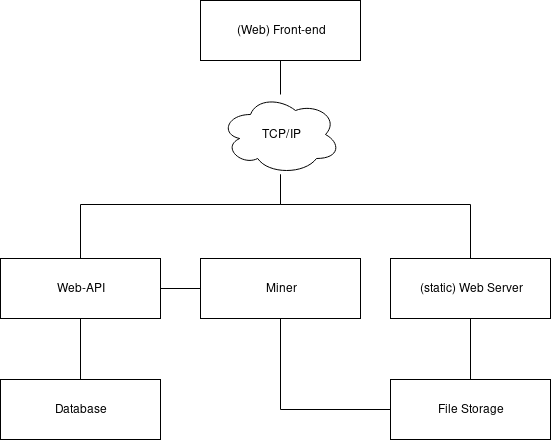
\includegraphics[width=12cm]{images/highlevelarchitecture.png}
    \caption{High-level logical view of the architecture.}
    \label{fig:highlevelview}
\end{figure}


\subsection{Deployment View}
\subsubsection{Production}
The following paragraphs describe how the modules outlined in the previous chapter are built and how they can be mapped to a physical view along with physical constraints they introduce. This section will introduce the technologies that were used for the modules since these are relevant for the description of the deployment and constraints, however their evaluation will be described in the next chapter.
All of the modules described in the application tier of the logical view will run in a Docker service which will together form a Docker stack. This stack will require two Docker volumes for persistency to store the analysis files and the database. The services will expose two web-services over the network, one for the web API and one for the front-end application.

The simplest service will be the \textbf{analysis web server} and \textbf{frontend web server}. Both will be based on a simple nginx web server which will thus be purely third-party software that will be configured to our needs. Both web services can be scaled up by using multiple instances of the same Docker container, which brings the advantage of scaling up individual components. For example, if many people will access analysis file but only a few will upload new ones through the Web API service one can simply scale up that web server. Both web servers will not deal with huge quantities of data, thus having a low-latency network will be more important for these web services. Finally, the analysis web server will need access to the storage volume that contains the analysed files which were the output of the data miner.

The next service which will be exposed to the outside over the network is the Web API. This is a bespoke RESTful API built using Express.js that runs on Node.js. This module allows new network captures to be uploaded and analysed. It will also give meta-information about existing network capture files that are analysed. It will therefore require an internal connection to the database and to the packet miner. The external network connection should provide a large bandwidth since the network capture files can be easily surpass multiple gigabytes. Otherwise this service will require few resources since the evaluation of libraries revealed that even large files can be uploaded with just around 20 MB of memory. A few gigabytes need to be provided as temporary storage for uploading files without loading them into the memory. Since the service itself contains no persisted state it can also be scaled up by running multiple instances behind a load balancer.

The packet miner is the module that will be invoked by the Web API to process a raw network capture file. This bespoke module will be built on the Node.js platform and interact with libpcap. The output of this module needs to be written into the file storage and the result of an analysis needs to be reported back to the Web API module so that this module can store it into the database. Besides fast access to the raw capture files this service will be demanding in processing power but will not have high memory demands. This was revealed by exploratively building a prototype, as described in section \ref{scaleandschema}. It has to be noted that the actual memory usage depends on the analysis that is done. This means that the way how the system will be extended will have a greater influence on memory consumption than the size of the network capture files. If one were to write very demanding analyses one could still scale up the overall service by running parallel instances.

 The last service is the database that is used by the Web API. It contains metadata such as the previously analysed files. We assume that it will not require large amounts of file storage since the actual analysis results are written directly to the file system. The database service will be a simple MongoDB instance that will not be parallelized.
 
 The modules described above, their network connections and persitency volumes are shown in figure \ref{fig:deploymentviewprod}


\begin{figure}
    \centering
    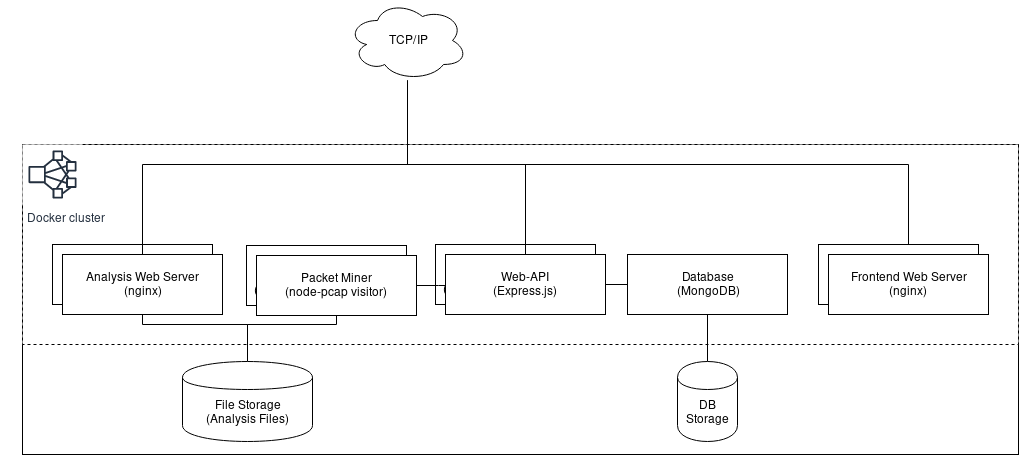
\includegraphics[width=16cm]{images/deploymentviewprod.png}
    \caption{Deployment view view of the final architecture.}
    \label{fig:deploymentviewprod}
\end{figure}


\subsubsection{Minimum Viable Product}
In order to build the system in an iterative manner we derived a simpler version of the architecture described in the previous section. This architecture is a pure simplification that is still compatible and should allow quicker prototyping and gathering of feedback. Since this is an intermediate (intermediary??) piece of work we will only describe it briefly.

To build a minimal version that can show the systems capabilities and gather feedback there would only be one service exposed and operated by us. This would be a Node.js based Express.js application that contains the RESTful API, a static webserver for the analysis files and an embedded database for metadata. The actual miner would be built in a separate Node.js module but run in the same process. Since in this version we are the only developers writing analysis modules we can easily optimize this part so that the overall memory cap (??) of 1.5 GB is not an issue. This configuration also only requires one file storage volume for both database and analysis files. Once we intend to optimize and extend the system we can pull the modules apart into their own Docker containers and replace some of the parts such as the Webserver and database with thirdparty technology such as nginx and Mongodb.
For convenience the frontend application can directly be hosted by GitHub pages which provides fast integration into the continuos delivery process. Since GitHub pages provides free https certificates and has CORS configured properly it provides all requirements for the frontend web application.

Figure \ref{fig:deploymentviewmvp} visualizes which services will be run by whom and how the application stack is composed.

\begin{figure}
    \centering
    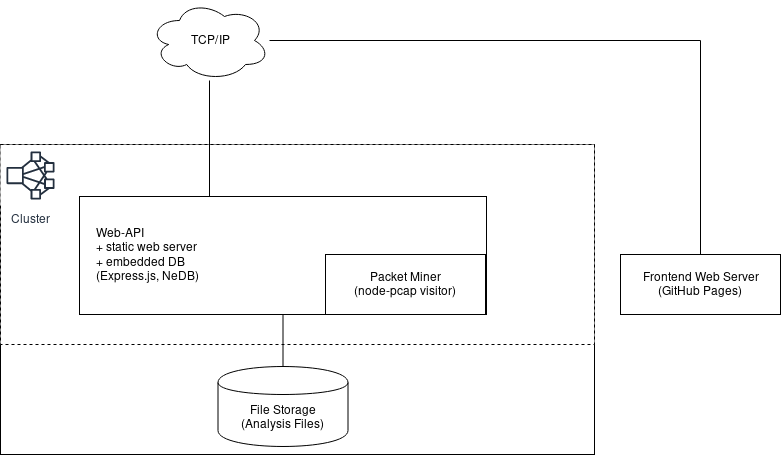
\includegraphics[width=16cm]{images/deploymentviewmvp.png}
    \caption{Deployment view view of the minimal architecture.}
    \label{fig:deploymentviewmvp}
\end{figure}

\subsection{Backend Development View}
The previous section has already described which services exist in the backend and on which technologies they are based on. Since this architecture contains both bespoke parts and third-party software we will not describe the design of their internals but rather just outline the most relevant relevant questions and challenges that were faced when building the architecture.

\subsubsection{Network capture decoding}
The biggest decision when designing the architecture was which library to use for network capture decoding. The evaluation of possible libraries was explored in the beginning as described in \ref{librariesandtooling}. The findings of our exploration was that we would either use the Node.js based node\_pcap library or a Java-based library. Since this module is probably the most important for our project this decision became central since it would decide the overall platform used. For example we would rather not build build the miner in Java and the Web API in JavaScript.
Finally we decided to use the Node.js based library for the following reasons:
\begin{itemize}
    \item The exploration showed that the Node.js based solution is performant enough for our implementation. We found no problems decoding capture files that are several gigabytes large with less than a hundred megabytes of memory consumption. 
    \item The exploration showed that the analysis performed after/ during (??) the decoding will require careful optimization. We both felt like doing event-based processing that works for very large files was more natural and simpler in Node.js
    \item We were both already familiar with Node.js and other related technologies. In a way we may have prioritized development speed over execution performance.
    \item Node.js is frequently used for rapid protoyping (source??). Since one of our use cases focuses on easy extension of adhoc analysis we expect that other developers might find this technology stack easy to work with.
\end{itemize}{}
\subsubsection{Persistence}
Once we wrote the first packet decoders we were able to reason about the type of persistence technology to be used. We figured that it makes sense to have metadata persisted in a database and analysis results stored as plain JSON files. The reason for this is that the analysis modules can stay independent of a common data model and that it is simpler to do stream processing on files. We found no problems with this decision since there is little aggregation performed after the mining has completed. This means that the output of the miner should already be optimized so that it can be simply used as input by the visualizations in the frontend.
\subsubsection{File uploading}
Since we have already decided that the packet decoder was built in Node.js we wanted to use the Node.js for other services as well such as the Web API which allows file uploading. For Node.js many file uploading middleware exists, however only a few make it possible to have large files being uploaded using a stream-based approach. This requirement was important because it does not make sense to optimize the packet decoder for large files if they can't be uploaded. Finally we found that Express.js, a web-framework for Node.js, has support for this feature in a configurable way, so we went ahead to incorporate this as a design decision into the architecture. 
\subsubsection{Orchestrating Packet Visitors}
A complex part of the code was the orchestration of different visitors that may access the same stream of decoded packets. A visitor is a independent piece of code which receives some packets it is interested in and produces some intermediary and final result. For example one visitor could count the ratio of packet that are UDP and TCP while another may count IP protocol versions. The core issues included:

\begin{enumerate}
    \item The visitors, which may be independent, may need asynchronous setup. For example an analysis of autonomous systems behind source IPs might need to setup a database connection first.
    \item The visitors might do asynchronous post-processing, such as the computation of metrics.
    \item The visitors might store intermediary data differently.
    \item The packet decoding module emits very abstract events such as "packet", "start" and "end". Since each visitor is interested in different packet types this would lead to logic being duplicated across these visitors. For example, both a UDP and TCP port analysis visitor would implement logic to parse up until the transport layer.
    \item Running the actual packet decoding should happen centralized, independent of the visitors. However the visitors must be synchronized to this.
\end{enumerate}{}

The first design decision that was made in this architecture was to write an intermediary EventEmitter (src??) that would listen to the three events emitted by node\_pcap and would generate more concrete events. This included the following:
\begin{itemize}
    \item One event being emitted per layer in the TCP/IP model
    \item One event being emitted per protocl in the TCP/IP model. This covered the protocols Ethernet, IPv4, IPv6, UDP, TCP and all well-known application level protocols based on destination port.
    \item Events for frequently used properties of the former protocol. For example, a visitor may just listen to the destination ports being emitted, without caring if they stem from UDP or TCP packets.
\end{itemize}{}
This was implemented as a class \textit{PcapParserFacade} and eliminated issue 4. The remaining issues all required one implementation goal (??), namely the orchestration of an asynchronous visiting of the packets by independent visitors with support for setup, parsing and post-parsing actions. This was achieved using two classes that can then be used by subclassing and composition.

The first class is a \textit{GenericPcapAnalyser} which is similar to an abstract class. This class expects a  \textit{PcapParserFacade} composed and has two asynchronous functions that can be used to hook the minimal logic. First a \textit{setUp} function allows that all events can be registered to the facade that is composed. It may also be used to perform asynchronous logic such as a database connection. The asynchronous nature makes it easy to allow the client of this class to synchronize these setUp functions.
The start of the packet decoding in the Facade will be called from outside by the client, which also listens to the termination of the decoding. Once this decoding has finished the client can asynchronously instruct the subclasses of \textit{GenericPcapAnalyser} to perform their post-analysis steps and write them to files.


 \subsection{Frontend Development View}
 This section presents the components chosen and thought processes behind choosing them for the frontend application the users will interact with.  
 \subsubsection{Base Web Application}
 After considering multiple frameworks, it was decided that we use Vue.js as a base framework for the application. Factors that supported this decision was the fact that we both were familiar with the framework already, meaning we could quickly build a working prototype and the Node.js ecosystem provided many Vue.js-specific that makes working with it easier. Other frameworks or development method that were considered included React and templating WebComponents using lit-element. We decided against these 2 methods, because we did not have any experience using them, meaning a considerable amount of time would have been spent getting familiar with them. While the lit-element/WebComponent approach would have been interesting from a technology standpoint, the ecosystem at the point of writing this report was just not at a point where using it was a hassle-free experience, for example Material Components were not yet fully implemented in WebComponent format.
 
 Vue.js allows the creation of Single Page Applications, which makes the dynamic loading of the applications possible, instead of needing to perform a full web-page reload for every action performed.
 \subsubsection{Grid-Layout Engine}
 Since the \emph{Dashboard} component of the application relies on a configurable grid, that can re-arrange its tiles automatically, a grid-layouting engine is required. Our requirements for such an engine included:
 \begin{enumerate}
    \item The tiles inside of a grid should be rearrangeable using drag and drop controls.
    \item The vertical size of the grid should be configurable during run-time.
    \item The size of the library should be as small as possible to prevent bloating the frontend application's total size.
    \item Sorting and Filtering should be supported or built-into the library.
    \item The grid should react to changes in the number of tiles, such as deletion of elements and react accordingly, as well as the addition of new tiles.
\end{enumerate}{}
After evaluating multiple libraries, we decided to use Muuri, a javascript-based grid-system. Other libraries that were considered included Gridstack.js and jQuery Shapeshift, but were decided against, since they either did not support the features described in our requirements or were considered "too heavy" in terms of size. The two mentioned alternatives also required jQuery which significantly increases an application's size and for our use-case would not see any use besides for this layout engine.
Muuri supports the sorting and filtering of elements out of the box and also lets a user define their own arrangement algorithm, should the default one be unsatisfactory. 
 \subsubsection{Components}
 To provide a unified design for the application and prevent us from developing and designing a user interface from scratch, it was decided that reusable components will be used. Since the material design guidelines provide an in depth explanation on how each available component should be used to build an application that is both familiar to use and visually consistent, it was decided to use a component-library that is styled using material design. Because the framework we used is Vue.js, a requirement was that the components should be supported by or built for Vue.js, so that they can be included easily into the application. We decided to use Vue Material because of the ability to include only the required components versus needing to import the whole component library, as is the case with Vuetify, which was also larger in size overall. The usage of such a library makes it easy to just import for example a tabbed layout without needing to spend unnecessary time configuring CSS and HTML.
 \subsubsection{Visualization and Charting Libraries}
 \subsubsection{Progressive Web App}

\chapter{Design and Implementation}
